\section{Lademodi}
Der Peugeot konnte auf zwei verschiedene Arten geladen werden. Zum einen besitzt er ein internes Ladegerät. Mit einem Hilfskabel kann also die Verbindung zum $230$ VAC-Netz hergestellt werden, dessen Spannung im Peugeot selbst auf die benötigte Gleichspannung umgesetzt wird. Alternativ kann unter Umgehung des internen Gleichrichters direkt mit Gleichstrom geladen werden, was höhere Ladeleistungen ermöglicht.

\paragraph{Laden am 230 VAC-Netz}
Zum Anschluss an Wechselspannungsnetz ist ein Hilfskabel nötig. Dieses Hilfskabel bildet zum einen den Übergang zwischen den verschiedenen Steckersystemen, zum anderen ist in ihm auch eine elektrische Schaltung eingebaut. Diese findet ihren Platz in einer Box in der Mitte des Kabels. Diese Schaltung übernimmt dabei sowohl Schutzaufgaben (Überspannungs- und Überstromschutz), als auch die Kommunikation mit dem Fahrzeug. So teilt die Schaltung dem Fahrzeug den maximal beziehbaren Strom mit (dieser ist ja unter Umständen durch die verwendete Steckdose bestimmt). Ausserdem sind in dieser Box mehrere Leuchtdioden verbaut, die den Zustand des Fahrzeuges sowie eventuelle Fehler anzeigen. Das vorliegende Hilfskabel ist für eine haushaltsübliche Steckdose mit $230$ VAC und $10$ A gedacht, es gibt jedoch insbesondere bei öffentlichen Ladestationen auch stärkere Anschlüsse, welche Dreiphasenwechselstrom übertragen. Dieses Hilfskabel mit Box ist in Abbildung \ref{fig:Hilfskabel} zu sehen:

\begin{figure}[h]
	\centering
		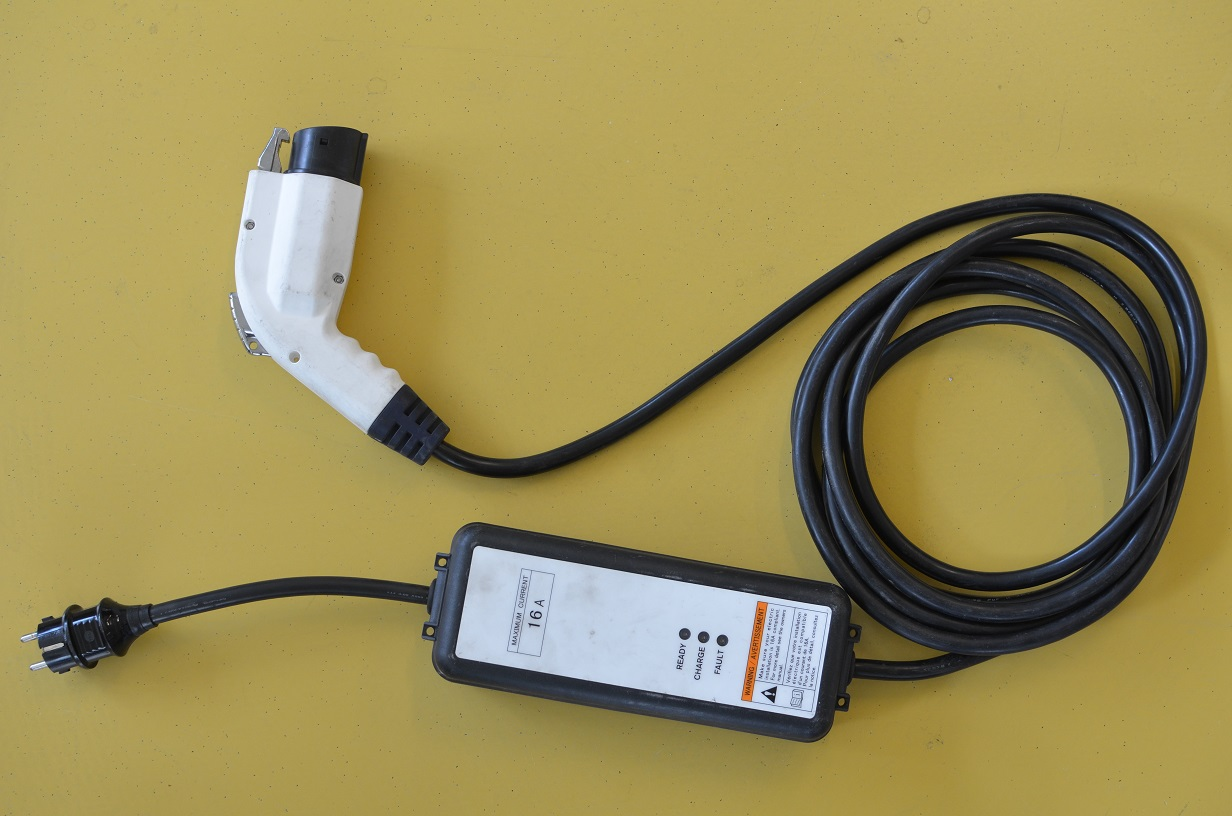
\includegraphics[width=0.80\textwidth]{images/Hilfskabel.JPG}
	\caption{Das verwendete Hilfskabel zum Laden mit $230$ VAC}
	\label{fig:Hilfskabel}
\end{figure}

Bei dieser Ladeart ist das gesamte Ladegerät innerhalb des Peugeots untergebracht. Auf dieses Ladegerät soll folgend eingegangen werden, zuerst sollen jedoch die Funktionen des Ladegerätes mithilfe von Abbildung \ref{fig:Laden_Peugeot} erläutert werden:

\begin{figure}[h]
	\centering
		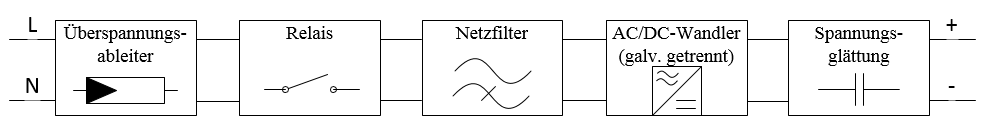
\includegraphics[width=1.00\textwidth]{images/Laden_Peugeot.PNG}
	\caption{Ablauf beim Laden des Peugeots am $230$ VAC Netz}
	\label{fig:Laden_Peugeot}
\end{figure}

Am Beginn steht die Schutzschaltung im Hilfskabel, welches bereits vorgestellt wurde. Das erste im Fahrzeug befindliche Bauteil ist ein Hauptrelais, welches die Ladung des Fahrzeuges ein- und ausschalten kann. Dieses Relais kann auch über das Hilfskabel geschaltet werden, sodass bei einem externen Fehler die Ladung abgebrochen werden kann. Als erste Stufe der eigentlichen Schaltung kann das Netzfilter gesehen werden. Mit Hilfe von Spulen und Kondensatoren sorgt dieses dafür, dass möglichst wenig Blindleistung aus dem Netz bezogen wird. Diese Blindleistung wird nämlich von dem Diodengleichrichter erzeugt, der dem Filter folgt. Diese Wechselspannung wird durch den Gleichspannungswandler, welcher nachfolgend noch detaillierter vorgestellt wird, auf den zur Batterie passenden Wert gebracht. Am Ende erfolgt noch eine Glättung der Ausgangsspannung, dies erfolgt mittels eines Kondensators.

Die Ausgangsspannung der Diodenbrücke weist mehrere Nachteile auf. Die grössten Nachteile sind die fehlende galvanische Trennung, die proportionale Abhängigkeit zur Netzspannung sowie die fehlende Möglichkeit zur Regelung. Ausserdem entspricht der Wert dieser Spannung nicht dem Wert, welcher die Batterie benötigt. Aus all diesen Gründen ist zwischen dem Diodengleichrichter und der Batterie ein Gleichspannungswandler eingebaut, der die zuvor beschriebenen Nachteile eliminiert. Die Schaltung des Starkstrompfades ist in Abbildung \ref{fig:Ladegeraet_Peugeot} abgebildet:

\begin{figure}[h]
	\centering
		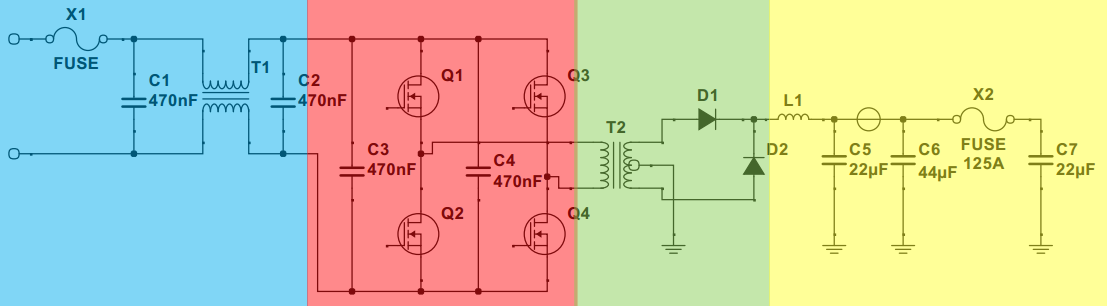
\includegraphics[width=1.00\textwidth]{images/Ladegeraet_Peugeot.PNG}
	\caption{Gleichspannungswandler im Ladegerät des Peugeots}
	\label{fig:Ladegeraet_Peugeot}
\end{figure}

Auch bei dieser Schaltung erfolgt eine eingangsseitige Glättung durch ein Filter, in der Abbildung blau dargestellt. Da die Eingangsspannung jedoch direkt von der Diodenbrücke, die bereits über eine kapazitive Glättung verfügt, erfolgt, konnte der Sinn dieses Filters nicht geklärt werden. Eine Idee wäre jedoch, dass unter Umgehung des Diodengleichrichters direkt mit einer Gleichspannung gespiesen werden kann. Die beiden Kondensatoren sorgen für gleichmässige Spannungen am Ein- und Ausgang, die gekoppelten Spulen sorgen dafür, dass bei sich schnell ändernden Strömen eine Gegenspannung einstellt.

Im roten Bereich befinden sich die vier Leistungs-MOSFETs vom Typ 2SK3697 \cite{2sk3697}. Diese vier Halbleiter erzeugen aus der Gleichspannung wieder eine Wechselspannung, allerdings mit deutlich höherer Frequenz als die Netzfrequenz. Dadurch kann der nachfolgende Transformator verkleinert ausgeführt werden. Parallel zu jeder Halbbrücke ist jeweils ein Kondensator eingebaut, der Spannungsabfälle bei den Schaltvorgängen abdämpft. Diese Wechselspannung kann durch Polaritätswechsel der Gleichspannung erzeugt werden, indem zwischen den Schaltzuständen $Q_1$ und $Q_4$ eingeschaltet und $Q_2$ und $Q_3$ eingeschaltet gewechselt wird. Sind die beiden oberen oder unteren Transistoren eingeschaltet, so ist die Ausgangsspannung der Brücke $0$ V. Durch abwechselnde Benutzung der Schaltzustände kann also sowohl die Frequenz als auch die Spannung der Brücke verändert werden, begrenzt wird dies lediglich durch die maximale Schaltfrequenz der Transistoren und der eingangsseitigen Gleichspannung.

Um eine galvanische Trennung und eventuell auch eine Spannungsanpassung zu ermöglichen, ist die grün hinterlegte Transformatorenschaltung eingebaut. Die Mittenanzapfung mit den beiden Dioden sorgt dafür, dass beide Halbwellen wieder gleichgerichtet werden können (im Vergleich zu einer Diodenbrücke können aber zwei Dioden eingespart werden). Dadurch kann der Eisenkern gut entmagnetisiert werden. Die induzierte Spannung entsteht je nach Polarität in der oberen oder der unteren Halbwicklung.

Auch ausgangsseitig wird die erhaltene Spannung geglättet, da sie ja vom Transformator her eine Welligkeit aufweist. Dies ist im gelben Bereich gezeigt und geschieht durch eine Spule und mehrere Kondensatoren. Nach dem ersten Tiefpass folgt ausserdem eine Strommessung, mit welcher schlussendlich die Regelung der MOSFETs beeinflusst wird. Ausserdem ist ausgangsseitig noch eine handelsübliche Kfz-Streifensicherung verbaut. Wird der Nennstrom dieser Sicherung ($125$ A) und auch die Abmessungen der übrigen Schaltungsteile berücksichtigt, so sieht man sehr gut, dass diese Schaltung für höhere Ströme als die $10$ A des Hilfskabel ausgelegt ist. Auch die aktive Wasserkühlung der gesamten Schaltung deutet dies an. So gibt Peugeot für das Modelljahr 2011 an, dass die $16.28$ kWh Batterie innerhalb von 20 Minuten zur Hälfte geladen werden kann \cite{ion}. Dies enspricht einer Ladeleistung von $24.42$ kW, wobei bei einem idealen Gleichrichter auf der Wechselspannungsseite ein Strom von $35.39$ A resultieren würde (dreiphasig). Werden zusätzlich Verluste und Blindleistung berücksichtigt, so erscheint ein Ladestrom von $40$ A, was einer Normsicherungsgrösse entsprechen würde, als realistisch.

\paragraph{Ladung mit Gleichstrom}
Das interne Netzgerät des Peugeots kann auch umgangen werden. Zu diesem Zweck besitzt der Peugeot einen sogenannten ChaDeMo-Anschluss, mit welchem direkt mittels Gleichstrom die Batterie geladen werden kann \cite{chademo}. Dieser Anschluss überträgt ausser dem Gleichstrom auch die Daten, die zur Kommunikation zwischen Fahrzeug und Ladegerät nötig sind. Neben Einschalt- und Schutzsignalen erfolgt der Datenaustausch über einen CAN-Bus, mit welchem das Fahrzeug der Ladestation den maximalen Ladestrom sowie den Ladezustand angibt.

Das Ladegerät kann in diesem Fall aus dem Auto ausgelagert werden, wodurch das Auto selbst unabhängig von der verwendeten Elektrizitätsform an der Eingangsseite wird. Dazu führen die beiden Starkstromleiter direkt von der Buchse zur Batterie, dazwischen ist keine Schaltung verbaut. Lediglich zum bereits angedeuteten Informationsaustausch zwischen dem Fahrzeug (in diesem Fall ausschliesslich dem Batteriemanagementsystem) und der Ladestation führen die Datenleitungen auf weitere Schaltungen. Dieses ChaDeMo-System ist auch für noch höhere Leistungen bis $100$ kW geeignet, wobei die meisten Ladestationen die Leistung auf $50$ kW begrenzen. Dies ist aber, verglichen mit dem internen Ladegerät, immer noch ungefähr die doppelte Leistung.

In beiden Fällen wird die Ladung durch das Batteriemanagementsystem des Peugeots überwacht und gesteuert. Da das ChaDeMo-Ladegerät auf jeden Fall mittels CAN-Bus angesteuert wird ist anzunehmen, dass auch die Kommunikation mit dem internen Ladegerät über diese Schnittstelle erfolgt.